\section{Thermodynamik} \marginpar{VL 12}

\begin{center}
    \emph{Wie passt die statistische Physik zur Thermodynamik?}
\end{center}

\begin{itemize}
    \item makroskopisch scheint alles deterministisch und ohne statistischen Ursprung
    \item Übertragung der thermodynamischen Konzepte auf mikroskopische Größen
    \begin{itemize}
        \item[]kein Problem: Impuls, Schwerpunkt, Teilchenzahl, innere Energie $U = \langle H \rangle$
        \item[]schwieriger: Temperatur, Druck, Wärme, thermodynamische Entropie 
    \end{itemize}
    \item Hauptsätze der Thermodynamik statistisch begründen
\end{itemize}

\subsection{0. Hauptsatz}
\begin{definition}{0. Hauptsatz}
    Zwei Systeme, die jeweils im thermischen Gleichgewicht mit einem dritten System sind, befinden sich auch untereinander im Gleichgewicht.
\end{definition}
Beschreibung in der statistischen Physik (kanonisches Ensemble):
\begin{itemize}
    \item zwei Systeme im Gleichgewicht zur Umgebung (3. System)
    \begin{itemize}
        \item[] System a:
        \begin{align}
            \varrho_a &= \frac{1}{Z_a(\beta_a)} e^{-\beta_a H_a} \\
            \underbrace{U_a}_{\langle E \rangle} &= - \pd{}{\beta_a} \ln\left( Z_a(\beta_a) \right) \: \Rightarrow \: \beta_a(U_a)
        \end{align}
        \item[] System b:
        \begin{align}
            \varrho_b &= \frac{1}{Z_b(\beta_b)} e^{- \beta_b H_b} \\
            U_a &= - \pd{}{\beta_b} \ln\left( Z_b(\beta_b) \right) \: \Rightarrow \: \beta_b(U_b)
        \end{align}
        \item[$\rightarrow$] $\beta_a \stackrel{?}{=} \beta_b$ 
    \end{itemize}
    \item Gesamtsystem $a+b$ in thermischen Kontakt:
    \begin{equation}
        H = H_a \otimes \mathds{1} + \mathds{1} \otimes H_b + V_{ab}
    \end{equation}
    \begin{itemize}
        \item[] $V_{ab}$ ist WW-Term, erlaubt Energieaustausch, $V_{ab} \ll H_a, H_b$ (beliebig klein)
    \end{itemize}
    \item[] Gesamtsystem an Umgebung gekoppelt: Gleichgewicht kanonisch
    \begin{align}
        \varrho_{a+b} &= \frac{e^{-\beta H}}{Z} = \frac{e^{-\beta\left(H_a \otimes \mathds{1} + \mathds{1} \otimes H_b + V_{ab}\right)}}{Z(\beta)} \\
        &\approx \frac{e^{-\beta H}}{Z} = \frac{e^{-\beta\left(H_a \otimes \mathds{1} + \mathds{1} \otimes H_b\right)}}{Z_a(\beta_a)\cdot Z_b(\beta_b)} \\
        \color{black!50} \text{NR: } Z(\beta) &= \color{black!50} \trace\left(e^{-\beta(\dots)}\right) = \sum_{m,n} \langle n,m| e^{-\beta(H_a \otimes \mathds{1} + \mathds{1} \otimes H_b )} \underbrace{|n,m\rangle}_{\ket{n}\ket{m}}\\
        \color{black!50} &= \color{black!50} \sum_{n,m} e^{-\beta H_n^a} e^{-\beta H_m^b} = Z_a(\beta) \cdot Z_b(\beta) \\
        &= \varrho_a(\beta) \otimes \varrho_b(\beta) \\
        &\Longrightarrow \beta = \beta_a = \beta_b
    \end{align}
\end{itemize}

\subsection{1. Hauptsatz}
\begin{definition}{1. Hauptsatz}
    \begin{itemize}
        \item[] Energieerhaltung
        \begin{equation}
            \Delta U = \Delta Q + \Delta W
        \end{equation}
        \item[] differentiell
        \begin{equation}
            dU = \delta Q + \delta W
        \end{equation}
        \begin{itemize}
            \item[]$dU$: exaktes Differential (totales Differential), vom Weg unabhängig
            \begin{itemize}
                \item[] Kreisprozess: $\oint \ dU = 0$
                \item[]
                \item[] $U$ Zustandsgröße, $U = \trace\left(\varrho H \right)$
            \end{itemize}
            \item[]$\delta Q, \delta W$: inexakte Differentiale, vom Weg abhängig
            \begin{itemize}
                \item[] Kreisprozess: $\oint \ \delta Q = -\oint \delta W \stackrel{i.A.}{\neq} 0$
                \item[]
                \item[] $Q,W$ keine Zustandsgrößen
            \end{itemize}
        \end{itemize}
    \end{itemize}
\end{definition}

\begin{beispiel}{Beispiel}
    zwei verschiedene Prozesse mit gleicher Zustandsänderung $\Delta U$
    \begin{enumerate}
        \item Gas wird Wärme $\delta Q = \Delta U$ zugeführt
        \item oszillierender Kolben (schnell): $\delta W = \Delta U$
    \end{enumerate}
    $\Rightarrow$ Erhöhung der inneren Energie, aber $\delta Q$ und $\delta W$ unbekannt, da keine Zustandsgrößen
\end{beispiel}

\paragraph{Wichtige Zustandsänderungen}
\begin{itemize}
    \item \emph{quasistatisch}: so langsam, dass immer im Gleichgewicht
    \item \emph{adiabatisch}: bei thermischer Isolation
\end{itemize}

\subsubsection{Was ist Wärme?}
\begin{itemize}
    \item System sei sei durch festes $H$ beschrieben, d.h. es wird keine Arbeit zugeführt ($\delta W = 0$)
    \item Kopplung an Umgebung (Wärmeübertragung) ändert $\varrho$
    \begin{align}
        U &= \trace\left(\varrho H\right) \stackrel{G.G.}{=} \sum_n p_n E_n \\
        dU &= \underbrace{\trace(d\varrho \: H)}_{\delta Q} + \underbrace{\trace(\varrho \: dH)}_{\delta W \text{ (hier = 0)}} \\
        \rightarrow \delta Q = \trace(d\varrho \: H) = \sum_n dp_n E_n
    \end{align}
\end{itemize}

Wärmezufuhr entspricht Umverteilung der Wahrscheinlichkeiten $p_n$ für Mikrozustände (während Wärmeübertragung $\rightarrow$ kein Gleichgewicht)\\
$\longrightarrow$ meist nicht reversibel


\subsubsection{Was ist Arbeit?}
\begin{itemize}
    \item System tauscht keine Wärme aus ($\delta Q = 0$)
    \item makroskopische Variablen $\xi_i$ werden extrem geändert
    \begin{align}
        H &= H(\{\xi_i\}) \rightarrow dH = \sum_i \underbrace{\pd{H}{\xi_i}}_{\chi_i} d\xi_i \\
        dU &= \underbrace{\trace(d\varrho \: H)}_{\delta Q \text{ (hier = 0)}} + \underbrace{\trace(\varrho \: dH)}_{\delta W} \\
        \delta W &= \color{black!50} \underbrace{\color{black}\trace(\varrho \: dH) \color{black!50}} \color{black} = \sum_n p_n \ dE_n \\
        & \color{black!50} \trace(\varrho \sum_i \chi_i \ d\xi_i) = \sum_i \trace(\varrho \chi_i) d\xi_i = \sum_i \langle \chi_i \rangle d\xi_i
    \end{align}
\end{itemize}

\begin{center}
    \begin{tikzpicture}[scale=0.9]
        \draw[thick] (0,0) -- (5,0) -- (5,2) -- (0,2);
        \filldraw[pattern=north east lines] (1,2) rectangle (0.75,0) node[anchor= north west]{$\xi$};
        \draw[<-,thick] (1.5,1) -- (0,1) node[anchor=east]{$\Vec{F}$};
    \end{tikzpicture}
\end{center}
\begin{equation}
    \delta W = F \ ds = - p \ dV = \mu \ dN
\end{equation}
\vspace{1cm}
\begin{itemize}
    \item[$\longrightarrow$] meist reversibel
    \item[$\longrightarrow$] Wärmezufuhr nicht reversibel 
\end{itemize}



\subsubsection{Exakte und inexakte Differentiale}
\paragraph{Exaktes (vollständiges, totales) Differential:}

Sei $F(x,y)$ Funktionen von 2 Veränderlichen
\begin{wrapfigure}{l}{2cm}
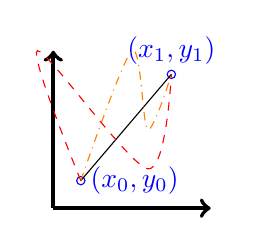
\begin{tikzpicture}
\coordinate (a) at (0.35,0.35);
\node[right, color=blue] at (a) {$(x_0,y_0)$};
\coordinate (b) at (1.5,1.7);
\node[above, color=blue] at (b) {$(x_1,y_1)$};
\draw[blue] (a) circle (1.5pt);
\draw[blue] (b) circle (1.5pt);
\draw[->, line width =1.5pt] (0,0)--(2,0);
\draw[->, line width =1.5pt] (0,0)--(0,2);
\draw (a)--(b);
      \draw[dash dot,orange] plot [smooth] coordinates {(a) (1,2)  (1.2,1) (b)};
       \draw[dashed, red] plot [smooth] coordinates {(a) (-0.2,2)  (1.2,0.5) (b)};
\end{tikzpicture}
 \end{wrapfigure}
\begin{align}
    dF &= \pd{F(x,y)}{x} \, dx + \pd{F(x,y)}{y} \, dy \\
    \int_{x_0,y_0}^{x_1,y_1} dF &= F(x_1,y_1) - F(x_0,y_0) = \text{wegunabhängig}
\end{align}
\begin{equation}
    \frac{\partial^2 F(x,y)}{\partial y \partial x} \stackrel{\text{Satz v. Schwarz}}{=} \frac{\partial^2 F(x,y)}{\partial x \partial y}
\end{equation}

\paragraph{Inexaktes (unvollständiges) Differential:}
\begin{align}
    \delta G &= a(x,y) \ dx + b(x,y) \ dy \\
     \int_{x_0,y_0}^{x_1,y_1} \delta G &= \text{wegabhängig}\\
     \text{da } &\nexists G(x,y) \text{ mit } \pd{G(x,y)}{x} = a(x,y) \quad \pd{G(x,y)}{y} = b(x,y) \\
     \Big( &\text{außer falls } \pd{a}{y} = \pd{b}{x} \Leftrightarrow \frac{\partial^2 G(x,y)}{\partial y \partial x} = \frac{\partial^2 G(x,y)}{\partial x \partial y} \Leftrightarrow \exists G \Big)
\end{align}

Integrierender Faktor $I(x,y)$:
\begin{align}
    I(x,y) \ \delta G &= I(x,y) \ a(x,y) \ dx + I(x,y) \ b(x,y) \ dy \\
    &\text{mit } \pd{}{y}\left( I(x,y) \ a(x,y) \right) \stackrel{!}{=} \pd{}{x}\left( I(x,y) \ b(x,y) \right) \\
    &\Rightarrow \text{ exaktes Differential } dF = I(x,y) \delta G
\end{align}

\begin{beispiel}{Beispiel aus der Thermodynamik}
    \begin{equation}
        dS = \underbrace{\frac{1}{T}}_{\text{integrierender Faktor}} \quad \delta Q
    \end{equation}
\end{beispiel}


\subsection{2. Hauptsatz}\marginpar{VL 13}
Motivation: Energieerhaltung (1. HS) erlaubt viele Prozesse, die aber nicht vorkommen, z.B. $\text{Wärme} \longrightarrow \text{Energie}$

\begin{definition}{2. Hauptsatz}
    Äquvalente Formulierungen:
    \begin{itemize}
        \item Kelvin 1854:
        \begin{quote}
            Ein Prozess, dessen einziges Endergebnis ist, einer Quelle Wärme zu entziehen und in Arbeit zu verwandeln ist unmöglich.
        \end{quote}
        \item Clausius 1854:
        \begin{quote}
            Ein Prozess, dessen einziges Endergebnis ein Wärmetransfer von kalt nach warm ist, ist unmöglich.
        \end{quote}
        \item Carnot 1824:
        \begin{quote}
            Wirkungsgrad $\eta$ einer Wärmekraftmaschine mit zwei Wärmebädern $T_1 > T_2$:
            \begin{equation}
                \eta \leq \frac{T_1-T_2}{T_1} = 1- \frac{T_2}{T_1} 
            \end{equation}$\Longrightarrow$ absolute Temperatur
        \end{quote}
        \item Clausius 1865:
        \begin{quote}
            Im thermodynamischen Gleichgewicht wird ein System durch Temperatur $T$ und Entropie $S$ beschrieben. In eienm quasistatischen Prozess gilt:
            \begin{equation}
                dS = \frac{\delta Q}{T}
            \end{equation}
            2. HS: Jeder andere nicht quasistatische Weg von Gleichgewicht 1 zu Gleichgewicht 2 ist irreversibel:
            \begin{equation}
                S_2 - S_1 \geq \sum_j \int \frac{\overbrace{\delta Q}^{\text{Wärmemenge von Bad j}}}{\underbrace{T}_{\text{Temperatur von Bad j}}}
            \end{equation}
            Wärmeisoliertes System: $\delta Q = 0$
            \begin{equation}
                \Rightarrow S_2 \geq S_1 \qquad (\text{Entropie kann nicht abnehmen})
            \end{equation}
        \end{quote}
    \end{itemize}
\end{definition}

\paragraph{Bemerkung zu Temperatur und thermodynamischer Entropie $S_{th}$}
\begin{itemize}
    \item beide nur bis auf Faktor definiert
    \item $S_{th}$ nur bis auf additive Konstante definiert (wird im 3. HS festgelegt)
\end{itemize}

\paragraph{Zusammenhang Temperatur $T$ aus Thermodynamik und $\beta$ aus statistischer Physik:}
quasistatische Prozesse $\Longrightarrow$ $\varrho$ im Gleichgewicht
\begin{align}
    \varrho &= \frac{e^{-\beta H}}{Z} \qquad S = - k \trace(\varrho \ln(\varrho)) \\
    &\text{\color{black!50} geht, da in GG $\Rightarrow$ in EZ ausdrücken} \\
    \Rightarrow dS &= - k \trace(d\varrho \: \underbrace{\ln(\varrho)}_{-\ln(Z) - \beta H}) - \underbrace{ k \trace(d\varrho)}_{=0} \\
    &\color{black!50} \trace(\varrho) = 1 \Rightarrow \trace(d\varrho) = 0\\
    dS &= k \ln(Z) \underbrace{\trace(d\varrho)}_{=0} + k \beta \underbrace{\trace(d\varrho \: H)}_{\delta Q = T dS_{th}} \\
    dS &= k T \beta dS_{th} \\
    &\Longrightarrow \beta = \frac{1}{kT} \cdot \underbrace{const.}_{\text{wähle 1}} \qquad \text{und } \ S = S_{th} + const.
\end{align}
$\Longrightarrow$ Äquivalenz von $\beta, \ S$ und $T, \ S_{th}$ bis auf Faktor und additive Konstante bei der Entropie

\paragraph{Bemerkung:}
\begin{itemize}
    \item 2. HS für isoliertes System ($\delta Q = 0$): $dS \geq 0$
    \begin{itemize}
        \item[$\widehat{=}$] Prinzip der maximalen Entropie der statistischen Physik
    \end{itemize}
    \item Entropie im kanonischen Ensemble (\ref{sec.Kanonisches Ensemble})
    \begin{align}
        S(\langle E\rangle) &= k \ln(Z) + \underbrace{k \beta}_{\frac{1}{T}} \underbrace{\langle E \rangle}_{E} \\
        \pd{S(E)}{E} &= \frac{1}{T}\\
        &\text{Definition der Temperatur in der statistischen Physik}
    \end{align}
    \item Entropie im Großkanonischen Ensemble (\ref{sec.Großkanonisches Ensemble})
    \begin{align}
        S(\langle E \rangle, \langle N \rangle) &= k \ln(Z_G) + \underbrace{k \beta}_{\frac{1}{T}} \langle E \rangle + \underbrace{k \alpha}_{-\frac{1}{T} \mu} \langle N \rangle \\
        \pd{S(E,N)}{E} &= \frac{1}{T} \\
        \pd{S(E,N)}{N} &= - \frac{1}{T} \mu
    \end{align}
\end{itemize}

\subsection{3. Hauptsatz}
\begin{definition}{3. Hauptsatz}
    Nernst 1906:
    \begin{quote}
        Bei $T=0$ ist Entropie unabhängig von Parametern $\xi_i$ von $H(\{\xi_i\})$
    \end{quote}
    äquivalente Aussage:
    \begin{quote}
        Der absolute Temperatur-Nullpunkt ist mit endlicher Zahl von Schritten nicht erreichbar.
    \end{quote}
    Planck:
    \begin{quote}
    Wähle additive Konstante der Entropie so, dass $S_{th}(T=0) = 0$
    \end{quote}
    \begin{align}
        \Rightarrow S_{th} &= S \\
        p_m &= \frac{e^{-\beta E_m}}{\sum_n e^{-\beta E_n}} = \frac{e^{-\beta (E_m-E_0)}}{\sum_n e^{-\beta (E_n-E_0)}} \quad E_0 - \text{Grundzustandsenergie}\\
        p_m &\stackrel{T \to 0, \beta \to \infty}{\longrightarrow} \begin{cases}
            0 \quad, m > 0 \\ 1 \quad, m = 0
        \end{cases} \Rightarrow S = - k \sum_m p_m \ln(p_m) = 0 \\
        &\text{unabhängig von $E_m$, d.h. von Systemparametern $\xi_i$} \quad \checkmark \\
        &\text{\color{black!50} (funktioniert auch bei Entartung)}
    \end{align}
\end{definition}

\begin{beispiel}{Beispiel ideales Gas klassisch}
    \begin{align}
        S &= kN \left( \ln\left(\frac{V}{N \lambda^3}\right) + \frac{5}{2}\right) \quad \text{mit } \lambda = \frac{h}{\sqrt{2 \pi m k T}} \\
        &\Rightarrow S \stackrel{T\to 0} - \infty \\
        &\color{black!50} \Rightarrow \varrho(\Vec{q},\Vec{p}) = \frac{e^{-\beta H(\Vec{q},\Vec{p})}}{Z}\\
        &\color{black!50} \rightarrow \text{Wahrscheinlichkeitsdichte zieht sich auf Punkt im Phasenraum zusammen}\\
        &\color{black!50} \rightarrow \text{passt nicht mehr mit Planck-Zelle zusammen}\\
        &\rightarrow \text{Widerspruch zum 3. HS}\\
        &\Longrightarrow \text{q.m. Rechnung für $T\to 0$ notwendig!}
    \end{align}
\end{beispiel}

\subsection{Thermodynamischer Limes}
\begin{definition}{Thermodynamischer Limes}
\begin{itemize}
    \item System groß gegenüber mikroskopischen Abständen
    \item viele Teilchen $N\to \infty$, aber $\frac{N}{V}=const.$
    \item Oberflächeneffekte vernachlässigbar
    \item Form unwichtig, Volumen ausreichende Beschreibung
\end{itemize}

\paragraph{Extensive Variablen}:
\begin{itemize}
    \item[] proportional zum Volumen
    \begin{itemize}
        \item[Bsp.:] Teilchenzahl, Volumen, Entropie, Innere Energie, Masse, Impuls
    \end{itemize}
\end{itemize}

\paragraph{intensive Variablen}:
\begin{itemize}
    \item[] unveränderlich bei Volumenänderung
    \begin{itemize}
        \item[Bsp.:] Druck, Temperatur, Energie pro Teilchen $\frac{U}{N}$
    \end{itemize}
\end{itemize}
\end{definition}







\begin{beispiel}{Beispiel Extensivität der Entropie}
Entropie ist (lineare) homogen Funktion ersten Grades:
\begin{equation}
    S(\lambda U, \lambda V, \lambda N) = \lambda S(U,V,N)
\end{equation}
\begin{center}
    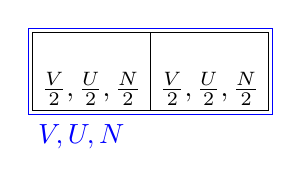
\begin{tikzpicture}
        \coordinate (lu) at (0.45,0.45);
        \coordinate (ro) at (3.55,1.55);
        \coordinate (lu1) at (0.5,0.5);
        \coordinate (lu2) at (2,0.5);
        \coordinate (ro1) at (2,1.5);
        \coordinate (ro2) at (3.5,1.5);
        \draw[blue] (lu) rectangle (ro);
        \draw (lu1) rectangle (ro1);
        \draw (lu2) rectangle (ro2);
        \node[below=8pt, right, blue] at (lu) {$V,U,N$};
        \node[above=8pt, right] at (lu1) {$\frac{V}{2},\frac{U}{2},\frac{N}{2}$};
        \node[above=8pt, right] at (lu2) {$\frac{V}{2},\frac{U}{2},\frac{N}{2}$};
    \end{tikzpicture}
\end{center}
\begin{equation}
    M_{\Delta}^1 \left(\frac{U}{2}\right) = M_{\Delta}^2 \left(\frac{U}{2}\right) \quad \text{und} \quad M_{\Delta} (U) \approx M_{\Delta}^1 \left(\frac{U}{2}\right) \cdot M_{\Delta}^2 \left(\frac{U}{2}\right)
\end{equation}
\begin{equation}
    S(V,U,N) = k \ln(M_{\Delta}(U)) = k \ln\left( M_{\Delta}^1 \left(\frac{U}{2}\right) \right) + k \ln\left( M_{\Delta}^2 \left(\frac{U}{2}\right) \right) = 2 S\left(\frac{V}{2},\frac{U}{2},\frac{N}{2} \right)
\end{equation}
\end{beispiel}

\begin{prop}{Gleichgewicht der Ensemble}
    Im thermodynamischen Limes sind die makroskopischen Eigenschaften von mikrokanonischem, kanonischem und großkanonischem Ensemble äquivalent.
\end{prop}


\subsection{Grundlegende Beziehungen der Thermodynamik}\marginpar{VL 14}
Zustandsgleichungen: Zusammenhang zwischen thermischen Zustandsgößen\\
Beispiel: Zustandsgröße $U\underbrace{(S, \quad V, \quad N)}_{\text{natürliche Zustandsvariablen}}$ ist ein thermisches Potential
\subsubsection{Fundamentalform}
1 HS:
\begin{align}
    dU=\underbrace{\delta Q}_{TdS} + \underbrace{\delta W}_{-pdV+\mu dN}
\end{align}
\begin{definition}{Gibbs'sche Fundamentalform}
    \begin{align}
        dU=TdS-pdV+\mu dN
    \end{align}
\end{definition}
mit den extensiven Größen $U,S,V,N$ und den internsiven Größen $T,p,\mu$\\
Die Zustandsgröße $U=U(S,V,N)$ ist eine thermodynamisches Potential und Funktion der Zustandsvariablen $S,V,N$ (natürliche Variablen)


\subsubsection{Physikalische Notation}
Partielle Ableitungen:
\begin{align}
    \pd{U(S,V,N)}{S}=\left(\pd{U}{S}\right)_{V,N}
\end{align}
Funktionen:
\begin{align}
    U(S,V,N),\overset{\sim}{U}(T,V,N),\overset{\approx}{U}(S,p,N),\overset{\approx}{\overset{\sim}{U}},\overset{\approx}{\overset{\approx}{U}},...
\end{align}
haben völlig verschiedene Abhängigkeiten von Argumenten: trotzdem ein Symbol $U'$!

$\left(\pd{U}{V}\right)_{T,N}$, $\pd{\Tilde{U}(T,V,N)}{V}$ und \underline{nicht} $\pd{U(S,V,N)}{V}$!


\subsubsection{Thermodynamische Kräfte}
$U(S,V,N)$ hat vollständiges Differential
\begin{align}
    dU=\left(\pd{U}{S}\right)_{V,N}dS + \left(\pd{U}{V}\right)_{S,N}dV + \left(\pd{U}{N}\right)_{S,V}dN
\end{align}
Vergleich mit Fundamentalform
\begin{definition}{Thermodynamische Kräfte}
    \begin{align}
        T=\left(\pd{U}{S}\right)_{V,N},\ p=-\left(\pd{U}{V}\right)_{S,N},\ \mu=\left(\pd{U}{N}\right)_{S,V}
    \end{align}
\end{definition}
Analogie zur Mechanik Potential $V(X)$, Kraft $F=-\pd{V}{x}$ wirkt auf $X$. hier th. Potential $U(S,V,N)$, th. Kraft $T=\left(\pd{U}{S}\right)_{V,N}$ wirkt auf S, $p=\left(\pd{U}{V}\right)_{S,N}$ wirkt auf V


\subsubsection{Maxwell Relationen}
\begin{align}
    T(S,V,N)=\left(\pd{U}{S}\right)_{V,N} \hspace{1cm} \text{und} \hspace{1cm} p(S,V,N)= -\left(\pd{U}{V}\right)_{S,N}
\end{align}
Thermodynamische Kräfte:
\begin{itemize}
    \item enthalten einzeln nicht die volle Information von $U$ (da Ableitung)
    \item sind nicht unabhängig, da 2. Ableitung vertauschen
        \begin{align}
            \pdv{U(S,V,N)}{V}{S}=\pdv{U(S,V,N)}{S}{V} &\Rightarrow \text{ Maxwell Relationen} 
        \end{align}
\end{itemize}



\begin{definition}{Maxwell-Relationen}
    \begin{align}
        \left(\pd{T}{V}\right)_{S,N} &= -\left(\pd{p}{S}\right)_{V,N}\\
        \left(\pd{T}{N}\right)_{S,V} &=\left(\pd{\mu}{S}\right)_{V,N}\\
        \left(\pd{\mu}{V}\right)_{S,N} &=-\left(\pd{p}{N}\right)_{S,V}\\
        &\dots
    \end{align}
\end{definition}


\subsubsection{Kalorische und thermische Zustandsgleichung}
Die Funktionen $U(S,V,N),T(S,V,N),p(S,V,N)$ sind schwer experimentell zu bestimmen, da $S$ nicht experimentell einstellbar.\\
Auflösen der Funktion $T(S,V)$ nach $S(T,V)$:
\begin{definition}{kalorische (1) und thermische (2) Zustandsgleichung}
    \begin{align}
        U(S,V) = U(S(T,V),V) \rightarrow U(T,V)\\
        p(S,V) = p(S(T,V),V) \rightarrow p(T,V)
    \end{align}
\end{definition}

\begin{beispiel}{Ideale einatomiges Gas}
    \begin{align}
        U(T,V,N)&=\frac{3}{2}NkT \hspace{1cm} \text{(unabh. von V)}\\
        p(T,V,N)&=\frac{NkT}{V}
    \end{align}
\end{beispiel}

\paragraph{Bemerkung:}
\begin{itemize}
    \item experimentell messbar
    \item enthalten einzeln nicht volle Information
    \item nicht unabhängig
\end{itemize}


\subsubsection{Entropie}
\begin{align}
    S(U,V,N) \; &\widehat{=} \; \text{in der Stat.Physik mikrokan. Ensemble} \\
    dS &= \frac{1}{T}dU + \frac{p}{T}dV-\frac{\mu}{T}dN\\
    &= \left(\pd{S}{U}\right)dU +\left(\pd{S}{V}\right)dV + \left(\pd{S}{N}\right)dN\\
    &\Rightarrow \left(\pd{S}{U}\right)_{V,N}=\frac{1}{T}, \left(\pd{S}{V}\right)_{U,N}=\frac{p}{T},\left(\pd{S}{N}\right)_{U,V}=-\frac{\mu}{T}
\end{align}

\begin{beispiel}{Ideales Gas}
aus stat Physik
    \begin{align}
        S=kN\left(\ln \frac{V}{N\lambda^3} + \frac{5}{2}\right) \quad \text{mit} \quad \lambda=\frac{h}{\sqrt{4\pi m U/(3N)}}
    \end{align}
    \begin{align}
        \frac{p}{T} &=\left(\pd{S}{V}\right)_{U,N}=kN\frac{1}{V} \quad \Rightarrow p=\frac{kNT}{V} \quad \checkmark\\
        \frac{1}{T} &=\left(\pd{S}{U}\right)_{V,N}=kN\frac{3}{2}\frac{1}{U} \quad \Rightarrow U=\frac{3}{2}kNT \quad \checkmark
    \end{align}
\end{beispiel}


\subsubsection{Euler-Gleichung, Gibbs-Duhen Relation}
Nutze Extensivität der inneren Energie (gilt nur für kurzreichweitige WW)
\begin{align}
    U(\lambda S,\lambda V, \lambda N)&=\lambda U(S,V,N)\\
    \eval{\dv{\lambda}}_{\lambda=1}&: \eval{\pd{U(S,V,N)}{S}}_{\lambda S,\lambda V,\lambda N, \lambda=1}S\\
    &= \underbrace{\left(\pd{U}{S}\right)_{V,N}}_{T} S+ \underbrace{\left(\pd{U}{V}\right)_{S,N}}_{-p} V + \underbrace{\left(\pd{U}{N}\right)_{S,V}}_{\mu} N = U(S,V,N)
\end{align}

\begin{definition}{Euler-Gleichung}
    \begin{align}
        U=TS-pV+\mu N
    \end{align}
    Differentielle Form
    \begin{align}
        dU=TdS + SdT - pdV - Vdp + \mu dN + Nd\mu
    \end{align}
    
\end{definition}
Subtraktion der Fundamentalform:
    \begin{align}
        dU = TdS -pdV + \mu dN
    \end{align}
\begin{definition}{Gibbs-Duhen-Relation}
    \begin{align}
        0= SdT - Vdp + Nd\mu
    \end{align}
\end{definition}
mit extensiven Größen $S,V,N$ und intensiven Größen $T,p,\mu$ $\leftarrow$ können nicht unabhängig voneinander variiert werden.


\subsection{Zustandsänderung und Materialgrößen}
\paragraph{Zustandsänderung (N=const)}
\begin{itemize}
    \item isotherm: $T=const$
    \item isochor: $V=const$
    \item isobar: $p=const$
    \item adiabatisch: $S=const,\delta Q = 0$
    \item quasistatisch : so langsam, das System immer im (partiellen) Gleichgewicht
    \item reversibel: $\Delta S_{Gesamt}=0$ (umkehrbar, hypothetischer Grenzfall, mind. quasistatisch)
\end{itemize}
\begin{beispiel}{quasistatisch (aber nicht reversibel)}
    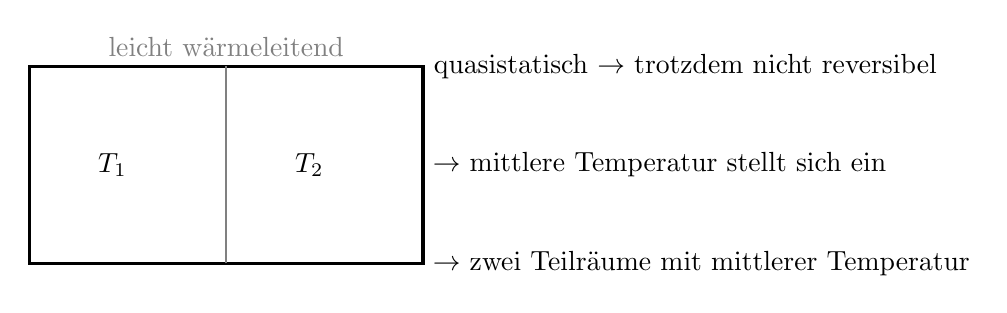
\begin{tikzpicture}[scale=0.5]
        \draw[very thick] (0,0) rectangle (10,5) node[anchor=west]{quasistatisch $\rightarrow$ trotzdem nicht reversibel};
        \draw[thick, black!50] (5,0) -- (5,5) node[anchor=south]{leicht wärmeleitend};
        \draw (10,2.5) node[anchor=west]{$\rightarrow$ mittlere Temperatur stellt sich ein};
        \draw (10,0) node[anchor=west]{$\rightarrow$ zwei Teilräume mit mittlerer Temperatur};
        \draw (1.5,2.5) node[anchor=west]{$T_1$};
        \draw (6.5,2.5) node[anchor=west]{$T_2$};
    \end{tikzpicture}
\end{beispiel}

\paragraph{Materialgößen}
\begin{itemize}
    \item Wärmekapazität bei konst Volumen
        \begin{align}
            c_v = \eval{\frac{\delta Q}{dT}}_V \overset{\delta Q=TdS}{=} T\left(\pd{S}{T}\right)_{V} \overset{\delta Q = dU + pdV}{=} \left(\pd{U}{T}\right)_{V}
        \end{align}
    \item Wärmekap. bei konst Druck
        \begin{align}
            c_p = \eval{\frac{\delta Q}{dT}}_p = T\left(\pd{S}{T}\right)_{p} = \left(\pd{U}{Tf}\right)_{p} + p\left(\pd{V}{T}\right)_{p}
        \end{align}
    \item isobarer (sogn. thermischer) Ausdehnungskoeffizient
    \begin{equation}
        \alpha = \frac{1}{V} \cdot \left( \pd{V}{T}\right)_p
    \end{equation}
    \item isochorer Spannungskoeffizient
    \begin{equation}
        \sigma = \frac{1}{p} \cdot \left(\pd{p}{T}\right)_V
    \end{equation}
    \item isotherme Kompressibilität
    \begin{equation}
        \kappa_T = - \frac{1}{V}\cdot \left(\pd{V}{p}\right)_T
    \end{equation}
    \item adiabatische Kompressibilität
    \begin{equation}
        \kappa_S = - \frac{1}{V} \cdot \left(\pd{V}{p}\right)_S
    \end{equation}

\end{itemize}

\newpage 
\subsection{Thermodynamische Potentiale}\marginpar{VL 15}
\subsubsection{Eigenschaften}
\begin{itemize}
    \item Zustandsgrößen mit Einheit Energie, insb. $U(S,V,N)$
    \item minimal im Gleichgewicht
    \item Abhängigkeit von natürlichen Zustandsvariablen
    \item partielle Ableitungen nach Zustandsvariablen sind einfache Ausdrücke
    \begin{itemize}
    \item[$\rightarrow$] thermodynamische Kräfte
    \end{itemize}
    \item volle thermodynamische Information
    \item alle 5 Potentiale sind gleichwertig, je nach physikalischer/chemischer Situation einfacher
\end{itemize}

\paragraph{Bemerkung} Entropie $S(U,V,N)$ ist thermodynamisches Potential im weiteren Sinne:
\begin{itemize}
    \item Einheit einer Entropie ($k_B$)
    \item maximal im Gleichgewicht
    \item partielle Ableitungen etwas komplizierter, z.B. $\left(\pd{S}{V}\right)_{U,N} = \frac{p}{T}$
\end{itemize}

\subsubsection{Freie Energie}
System mit festem $V,N$ in Umgebung mit $T$ \\
Ziel: Funktion von $T,V,N$ ($\widehat{=}$ kanonisches Ensemble mit $\beta = \frac{1}{kT}$)

\paragraph{Legendre-Transformation}

Funktion $f(x,t) \quad \rightarrow$ Ersetze $x$ durch $y$, $t$ unverändert; falls:
\begin{equation}
    y = \pdv{f(x,t)}{x} \quad \text{ und $f$ konvex } \frac{\partial^2 f(x,t)}{\partial x^2} > 0
\end{equation}
$y$ heißt konjugiert zu $x$ bezüglich $f$
\begin{equation}
    \rightarrow \text{Legendre-Transformierte  } \quad g(y,t):= f(x,t) - xy
\end{equation}
Eigenschaften:
\begin{itemize}
    \item hängt nur von $y,t$ ab, nicht von $x$
    \begin{equation}
        \frac{d}{dx} g(y,t) = \underbrace{\pdv{f(x,t)}{x}}_{=y} -y = 0 \quad \checkmark
    \end{equation}
    \item kein Informationsverlust
    \begin{proof}
        Rückkehr zu $f(x,t)$. Was ist $x$? $\pdv{g(y,t)}{y} = -x$ Nun machen wir die inverse Legendre-Transformation: $f(x,t) = g(y,t) + xy$
    \end{proof}
\end{itemize}

\subparagraph{Beispiel} klassische Mechanik
\begin{itemize}
    \item[] Lagrange-Funktion $L(q,\Dot{q})$ mit $p = \pdv{L}{\Dot{q}}$
    \item[$\Rightarrow$] Hamilton-Funktion: $-H(q,p) = L(q,\Dot{q}) - \Dot{q}p$ 
\end{itemize}
Anwendung auf thermodynamisches Potential $U(S,V,N)$
\begin{equation}
    T = \text{konj. Variable zu } S, \text{ da } T = \pdv{U}{S}
\end{equation}
Legendre-Transformation:
\begin{definition}{Freie Energie / Helmholtz-Potential}
\begin{equation}
    F(T,V,N) := U(S,V,N) - T \cdot S
\end{equation}
\end{definition}
\textbf{Bemerkung:}
\begin{itemize}
    \item hängt nicht von $S$ ab $\checkmark$
    \item volle thermodynamische Information enthalten
\end{itemize}


\subsubsection{Übersicht der thermodynamischen Potentiale}
natürliche Variablenpaare: $S \leftrightarrow T$, $V \leftrightarrow p$, $N \leftrightarrow \mu$

\begin{table}[h]
    \centering
    \caption{Übersicht zu den thermodynamischen Potentialen}
    \begin{tabular}{lcll}
         1 & $(S,V,N)$ & $U$ & innere Energie\\
         2 & $(T,V,N)$ & $F:= U - TS$ & freie Energie \\
         3 & $(S,p,N)$ & $H:= U + pV$ & Enthalpie \\
         4 & $(T,p,N)$ & $G := U - TS +pV$ & freie Enthalpie \\
         5 & $(S,V,\mu)$ & Teilchenaustausch + feste Entropie & $\rightarrow$ keine Anwendung\\
         6 & $(T,V,\mu)$ & $\Phi := U - TS - \mu N$ & großkanonisches Potential\\
         7 & $(S,p,\mu)$ & Teilchenaustausch + feste Entropie & $\rightarrow$ keine Anwendung\\
         8 & $(T,p,\mu)$ & $\Psi := U - TS + pV - \mu N = 0$ & $\rightarrow$ Euler-Gleichung\\
    \end{tabular}
    \label{tab:thermodynamische Potentiale}
\end{table}

\paragraph{Bemerkung:}
Nutze die Euler-Gleichung: $U = TS-pV+\mu N$, um Potentiale zu vereinfachen:
\begin{align}
    G(T,p,N) &= \mu N = \mu(T,p,N) \stackrel{\text{Extensivität}}{=} \mu(T,p) N \\
    \Phi(T,V,\mu) &= - pV \stackrel{\text{Extensivität}}{=} - p(T,\mu) V
\end{align}

\subsubsection{Beispiele für physikalische/chemische Situationen}
\begin{itemize}
    \item[U:] isoliertes System
    \item[F:] System im Wärmebad $T$
    \item[H:] chemische Reaktion bei konstantem Druck $p$
    \item[G:] chemische Reaktion bei konstantem $p$ und $T$
    \item[$\Phi$:] Adsorption an Oberflächen / Elektronengas in Metall 
\end{itemize}

\subsubsection{Differentielle Form}
\begin{align}
    \text{Fundamentalform} \quad dU &= T \cdot dS - p\cdot dV + \mu \cdot dN\\
    dF = dU - T \cdot dS - S \cdot dT \quad dF &= -S \cdot dT - p\cdot dV + \mu \cdot dN\\
    dH &= T \cdot dS + V\cdot dp + \mu \cdot dN \\
    dG &= -S \cdot dT + V \cdot dp + \mu \cdot dN \\
    d\Phi &= -S \cdot dT - p\cdot dV - N \cdot d\mu
\end{align}
    
\subsubsection{Thermodynamische Kräfte}
\begin{align}
    \left(\pdv{U}{S}\right)_{V,N} &= T, \quad \left(\pdv{U}{V}\right)_{S,N} = -p, \quad \left(\pdv{U}{N}\right)_{S,V} = \mu \\
    \left(\pdv{F}{T}\right)_{V,N} &= -S, \quad \left(\pdv{F}{V}\right)_{T,N} = -p, \quad \left(\pdv{F}{N}\right)_{T,V} = \mu \\
    \left(\pdv{H}{S}\right)_{p,N} &= T, \quad \left(\pdv{H}{p}\right)_{S,N} = V, \quad \left(\pdv{H}{N}\right)_{S,p} = \mu \\
    \left(\pdv{G}{T}\right)_{p,N} &= -S, \quad \left(\pdv{G}{p}\right)_{T,N} = V, \quad \left(\pdv{G}{N}\right)_{T,p} = \mu \\
    \left(\pdv{\Phi}{T}\right)_{V,\mu} &= -S, \quad \left(\pdv{\Phi}{V}\right)_{T,\mu} = -p, \quad \left(\pdv{\Phi}{\mu}\right)_{T,V} = -N
\end{align}

\subsubsection{Maxwell Relationen}
\begin{align}
    \frac{\partial^2 U(S,V,N)}{\partial V \partial S} &=\frac{\partial^2 U(S,V,N)}{\partial S\partial V} \Rightarrow \left(\pdv{T}{V}\right)_{S,N} = - \left(\pdv{p}{S}\right)_{V,N}\\
    \partial_{SN}^2 &= \partial_{NS}^2, \quad \partial_{VN}^2 = \partial_{NV}^2, \quad ...\\
    \frac{\partial^2 F(T,V,N)}{\partial V \partial T} &=\frac{\partial^2 F(T,V,N)}{\partial T\partial V} \Rightarrow -\left(\pdv{S}{V}\right)_{T,N} = - \left(\pdv{p}{T}\right)_{V,N}\\
    \partial_{TN}^2 &= \partial_{NT}^2, \quad \partial_{VN}^2 = \partial_{NV}^2, \quad ...
\end{align}

\subsubsection{Thermodynamisches Viereck (N=const)}
\textbf{Variablenpaare:} $S \leftrightarrow T$ und $V \leftrightarrow p$ \textbf{Potentiale:} $U,F,G,H$
\begin{center}
\begin{tikzpicture}[
roundnode/.style={circle, draw=blue!60, fill=blue!5, very thick, minimum size=7mm},
]
%Nodes
\node[roundnode]      (S)                    {S};
\node[roundnode]      (U)       [right=of S] {U};
\node[roundnode]      (V)       [right=of U] {V};
\node[roundnode]      (F)       [below=of V] {F};
\node[roundnode]      (T)       [below=of F] {T};
\node[roundnode]      (H)       [below=of S] {H};
\node[roundnode]      (p)       [below=of H] {p};
\node[roundnode]      (G)       [right=of p] {G};


%Lines
\draw[->,very thick] (S.south east) -- (T.north west);
\draw[->,very thick] (p.north east) -- (V.south west);
\end{tikzpicture}
\end{center}
\paragraph{Merkregel}
\begin{quote}
    dt.:  \underline{S}\underline{U}\underline{V} \underline{H}ilft \underline{F}ysikerinnen \underline{p}ei \underline{G}roßen \underline{T}aten.
\end{quote}
\begin{quote}
    engl.: \underline{G}ood \underline{p}hysicists \underline{H}ave \underline{S}tudied \underline{U}nder \underline{V}ery \underline{F}ine \underline{T}eachers.
\end{quote}
\paragraph{Beispiel}
$\Longrightarrow$ mit Potential anfangen, zur ableitenden Variable gehen und von dort dem Pfeil folgen, Pfeilrichtung ergibt Vorzeichen
\begin{align}
    \pdv{H}{S} &= T  \qquad \pdv{G}{p} = V\\
    \pdv{G}{T} &= -S \qquad \pdv{F}{V} = -p
\end{align}

\subsubsection{Verbindung zur statistischen Physik}
\paragraph{kanonisches Ensemble} (passt zur freien Energie $F$)
\begin{itemize}
    \item[] Dichteoperator:
    \begin{equation}
        \varrho = \frac{1}{Z} e^{-\beta H(V,N)} \quad \text{mit} \quad Z(\beta,V,N) = \trace\left(e^{-\beta H(V,N)}\right)
    \end{equation}
    \item[] Entropie:
    \begin{align}
        S(\beta,V,N) &= -k \trace(\varrho \ln(\varrho)) = k \ln(Z) + \underbrace{k \beta}_{\frac{1}{T}} \underbrace{\langle H \rangle}_{U}\\
        &\Rightarrow F = U-TS = -k T \ln(Z) \\
        &\fcolorbox{red}{white}{$\underbrace{F(T,V,N)}_{\text{Thermodyn.}} = \underbrace{-k T \ln\left(Z\left(\frac{1}{kT},V,N\right)\right)}_{\text{stat. Physik}}$}
    \end{align}
\end{itemize}

\paragraph{großkanonisches Ensemble}
\begin{equation}
    \fcolorbox{red}{white}{$\Phi(T,V,\mu) = -k T \ln\left(Z_G\left(\frac{1}{kT},V,\mu\right)\right)$}
\end{equation}

\paragraph{mikrokanonisches Ensemble}
\begin{equation}
    \fcolorbox{red}{white}{$S(U,V,N) = k \ln\left(Z_{mikro}(U,V,N)\right)$}
\end{equation}


\subsection{Stabilitätsbedingungen}\marginpar{VL 16}
\begin{itemize}
    \item thermische Stabilität:
    \begin{equation}
        c_V = \left(\pdv{U}{T}\right)_{V,N} > 0
    \end{equation}
    \item mechanische Stabilität:
    \begin{equation}
        \kappa_T = - \frac{1}{V} \left(\pdv{V}{p}\right)_{T,N} > 0
    \end{equation}
    \item chemische Stabilität:
    \begin{equation}
        \left(\pdv{N}{\mu}\right)_{T,V} > 0
    \end{equation}
\end{itemize}

\subsection{Phasengleichgewichte}
\begin{itemize}
    \item[] Stoff kann in verschiedenen Phasen auftreten (fest, flüssig, gasförmig) mit verschiedenen Eigenschaften (Dichte, Kompressibilität)
    \item[] Phasengleichgewicht: zwei oder mehr Phasen in Berührung und im Gleichgewicht
    \begin{itemize}
        \item[z.B.:] Eis + Wasserdampf + Wasser
        \item[] (inhomogenes System mit drei homogenen Teilsystemen)
    \end{itemize}
\end{itemize}

\paragraph{2 Phasen}
\begin{align}
    T_1 = T_2, \quad p_1 = p_2, \quad \mu_1 = \mu_2 \quad \Rightarrow \quad \mu_1(p,T) = \mu_2(p,T) \quad (\text{nur noch 1 Größe variabel})\\
    \Longrightarrow \text{ Koexistenzkurve (z.B. flüssig / gasförmig)}
\end{align}
\begin{center}
    \begin{tikzpicture}[scale=0.9]
        \begin{axis}[
        axis lines = left,
        axis line style={my axis},
        xmin=0, xmax = 6,
        ymin=0, ymax = 3.5,
        xtick=\empty, ytick=\empty,]
        \addplot[domain=1:5, samples=100, color=blue,]{exp(x/4)-0.5};
    \end{axis}
    \draw (7,0) node[anchor=west]{$T$};
    \draw (0,5.5) node[anchor=east]{$p$};
    \draw (5,4) node[anchor=west]{$\rightarrow$ Dampfdruckkurve};
    \draw[black!40] (3.5,2.5) node[anchor=west]{gasförmig};
    \draw[black!40] (2,3) node[anchor=west]{flüssig};
    \end{tikzpicture}
\end{center}

\paragraph{3 Phasen}
\begin{align}
    \mu_1(p,T) = \mu_2(p,T) = \mu_3(p,T) \\
    \Longrightarrow \text{ Tripelpunkt}\\
    (H_2O: \SI{0.01}{\celsius}, \SI{600}{\pascal})
\end{align}
\begin{center}
    \begin{tikzpicture}[scale=0.9]
        \begin{axis}[
        axis lines = left,
        axis line style={my axis},
        xmin=-1, xmax = 6,
        ymin=0, ymax = 3.5,
        xtick=\empty, ytick=\empty,]
        \addplot[domain=1:4.5, samples=100, color=blue,]{exp(x/4)-0.24};
        \addplot[domain=0:1, samples=100, color=green,]{1/x};
        \addplot[domain=-0.5:1, samples=100,]{exp(x/2)-0.6};
    \end{axis}
    \draw (7,0) node[anchor=west]{$T$};
    \draw (0,5.5) node[anchor=east]{$p$};
    \draw[blue] (5,4) node[anchor=west]{$\rightarrow$ Dampfdruckkurve};
    \draw (1,0.5) node[anchor=west]{$\rightarrow$ Sublimationsdruckkurve};
    \draw[green] (1.5,5.5) node[anchor=west]{$\rightarrow$ Schmelzdruckkurve};
    \draw[black!40] (4.5,2.5) node[anchor=west]{gasförmig};
    \draw[black!40] (2,4) node[anchor=west]{flüssig};
    \draw[black!40] (0,2) node[anchor=west]{fest};
    \filldraw[red] (1.95,1.7) circle (3pt) node[anchor=north west]{Tripelpunkt};
    \end{tikzpicture}
\end{center}

\subsubsection{Clausius-Clapeyron-Gleichung}
2 Phasen im Gleichgewicht
\begin{align}
    &\Rightarrow d\mu_1(p,T) = d\mu_2(p,T)\\
    \text{Gibbs-Duhem: } \quad &S dT - V dp + N d\mu = 0\\
    &\Rightarrow d\mu = - \underbrace{\frac{S}{N}}_{=: s} + \underbrace{\frac{V}{N}}_{=:v}\\
    &\Rightarrow -s_1 dT + v_1 dp = -s_2 dT + v_2 dp\\
    &\Rightarrow (s_2 -s_1) dT = (v_2 - v_1) dp\\
    &\text{mit: } q_{1\to2} = T (s_2-s_1) \\
    &\Longrightarrow \quad \fcolorbox{red}{white}{\Large$\frac{dp}{dT}= \frac{(s_2-s_1)}{(v_2 - v_1)} = \frac{q_{1\to2}}{T(v_2-v_1)}$} \quad \text{(Clausius Clapeyron)}
\end{align}

\begin{itemize}
    \item[$q_{1\to 2}$]: Wärme pro Teilchen, die bei Phasenumwandlung von 1 nach 2 zugeführt werden muss
    \item[] flüssig $\rightarrow$ gasförmig: Verdampfungswärme
    \item[] fest $\rightarrow$ flüssig: Schmelzwärme
    \item[] fest $\rightarrow$ gasförmig: Sublimationswärme
    \item[$\rightarrow$] latente (\enquote{versteckte}) Wärme
\end{itemize}

\paragraph{Beispiele}
\begin{itemize}
    \item Dampfdruckkurve:
    \begin{align}
        v_g &> v_f \quad \Rightarrow \quad \frac{dp}{dT} = \frac{q_{1\to2}}{T\cdot v_g} \\
        \text{ideales Gas: } pV &= NkT \quad \Rightarrow \quad v_g = \frac{V}{N} = \frac{kT}{p}\\
        \rightarrow \frac{dp}{dT} &= \frac{p}{T^2} \frac{q_{fl\to g}}{k}\\
        &\stackrel{TdV}{\Longrightarrow} \frac{dp}{p} = \frac{q_{fl\to g}}{k} \ \frac{dT}{T^2} \Rightarrow \quad \text{Annahme: $q_{fl \to g}$ nicht von $T$ abhängig}\\
        &\Rightarrow \ln(p)\Big\vert_{p_0}^p = \frac{q_{fl\to g}}{k} \left(-\frac{1}{T}\right)\Big\vert_{T_0}^T\\
        &\Rightarrow p(T) = p_0 \cdot e^{-\frac{q_{fl\to g}}{k}\left(\frac{1}{T}-\frac{1}{T_0}\right)}
    \end{align}
    \item Sublimationsdruckkurve:
    \begin{align}
        v_g \gg v_f \quad &\Rightarrow \quad \text{wie Dampfdruckkurve}\\
        &\rightarrow q_{fest\to g} > q_{fl \to g} \quad \Rightarrow \quad \frac{dp}{dT} \text{ steiler}
    \end{align}
    \begin{center}
    \begin{tikzpicture}[scale=0.4]
        \begin{axis}[
        axis lines = left,
        axis line style={my axis},
        xmin=-1, xmax = 6,
        ymin=0, ymax = 3.5,
        xtick=\empty, ytick=\empty,]
        \addplot[domain=1:4.5, samples=100,]{exp(x/4)-0.24};
        \addplot[domain=0:1, samples=100,]{1/x};
        \addplot[domain=-0.5:1, samples=100,]{exp(x/2)-0.6};
        \addplot[domain=0:3, samples=100, color=red,]{sqrt(x^3-1)+0.75};
    \end{axis}
    \draw (7,0) node[anchor=west]{$T$};
    \draw (0,5.5) node[anchor=east]{$p$};
    \draw[black!40] (4.5,2) node[anchor=west]{gasf};
    \draw[black!40] (3,4) node[anchor=west]{fl};
    \draw[black!40] (-0.3,2) node[anchor=west]{fest};
    \draw[red] (2.8,5) node[anchor=west]{$CO_2$};
    \filldraw (1.95,1.7) circle (3pt);
    \end{tikzpicture}
\end{center}
    \item Schmelzdruckkurve:
    \begin{align}
        v_{fest} \approx v_{fl} \quad &\Rightarrow \quad \frac{dp}{dt} \text{ ist sehr steil}\\
        \text{Wasser: } v_{fest} > v_{fl} \quad &\Rightarrow \quad \frac{dp}{dT} < 0\\
        \text{meist: } v_{fest} < v_{fl} \quad &\Rightarrow \quad \frac{dp}{dT} > 0\\
    \end{align}
\end{itemize}

\subsubsection{Phasenregel von Gibbs}
$K$ (Komponenten) verschiedene Stoffe jeweils in $P$ verschiedenen Phasen (fest, flüssig, gasförmig) im Gleichgewicht $\longrightarrow$ Wieviele Freiheitsgrade gibt es? bzw. Was ist de Zahl unabhängiger intensiver Variablen?
\begin{equation}
    \fcolorbox{red}{white}{\large F = 2 + K - P} \quad \text{Gibbs´sche Phasenregel}
\end{equation}

\paragraph{Beweis:} intensive Variablen: $T, \,p,$ Konzentrationen $\frac{N_k^i}{N^i}$ mit $N_k^i$ -k-te Komponente in Phase i und $N^i$ - Teilchen in Phase i
\begin{equation}
    \Longrightarrow 2 + K\cdot P \quad \text{ intensive Variablen}
\end{equation}
\begin{itemize}
    \item Abhängigkeiten
    \begin{itemize}
        \item alle Phasen $i = 1,...,P$:
        \begin{equation}
            \sum_{k=1}^K \frac{N_k^i}{N^i} = \frac{N^i}{N^i} = 1 \quad \Rightarrow \text{ P Abhängigkeiten}
        \end{equation}
        \item alle Komponenten $k = 1,...,K$
        \begin{equation}
            \mu_k^1 = \mu_k^2 = ... = \mu_k^P \quad \Rightarrow \quad (P-1) \cdot K \text{ Gleichungen}
        \end{equation}
        \begin{equation}
            \Rightarrow F = 2 + K\cdot P - (P + (P-1)\cdot K) = 2 + K - P \quad \checkmark
        \end{equation}
    \end{itemize}
\end{itemize}

\subparagraph{Beispiele:}
\begin{itemize}
    \item Wasser + Wasserdampf: $K=1$, $P=2$ $\Rightarrow \quad F=1 \quad \Rightarrow$ Dampfdruckkurve
    \item Tripelpunkt: $F=0$
\end{itemize}

\subsubsection{Van der Waals-Gas}
\begin{equation}
    \left(p+a\frac{N^2}{V^2}\right) \left(V-Nb\right) = NkT
\end{equation}
Korrektur der Zustandgleichung des idealen Gases aufgrund von Wechselwirkungen (beschreibt Phasenübergang flüssig $\rightarrow$ gasförmig $\widehat{=}$ Dampfdruckkurve)
\begin{itemize}
    \item[$Nb$] Volumen wird durch Eigenvolumen anderer Gasteilchen reduziert ($\propto N$)
    \item[$a\frac{N^2}{V^2}$] Druck wird erhöht durch Binnendruck anziehender Kräfte (Randteilchen werden nach innen gezogen $\rightarrow$ hoher Druck; $\frac{N}{V}$ im Volumen und $\frac{N}{V}$ an der Oberfläche)
\end{itemize}
$a, \, b > 0$ teilchenspezifische Parameter
\begin{equation}
    p(V,T) = \frac{NkT}{V-Nb} - a \frac{N^2}{V^2} \quad \Rightarrow \quad p(v,T) = \frac{kT}{v-b} - a \frac{1}{v^2}
\end{equation}
Isothermen im $p-V-$Diagramm:

\begin{center}
    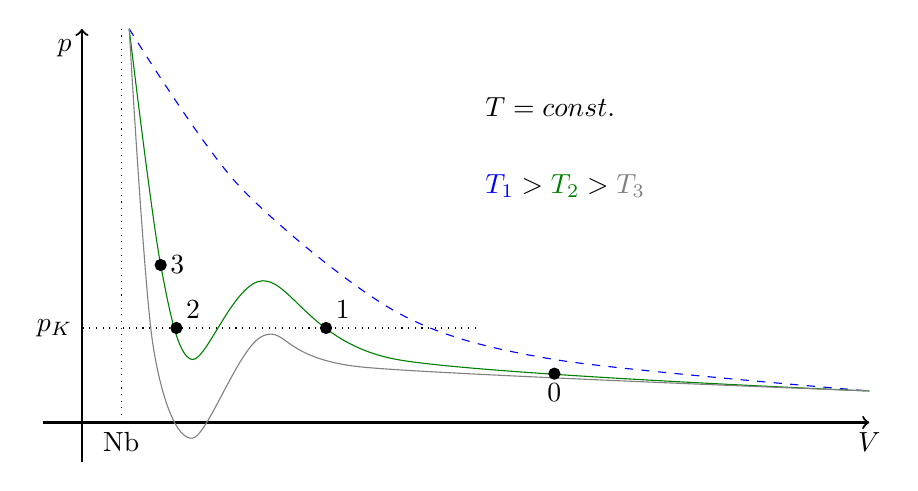
\begin{tikzpicture}
        \draw[->,thick] (-0.5,0) -- (10,0) node[anchor=north]{$V$};
        \draw[->,thick] (0,-0.5) -- (0,5) node[anchor=north east]{$p$};
        \draw[dotted] (0.5,5) -- (0.5,0) node[anchor=north]{Nb};
        \coordinate (a) at (0.6,5);
        \coordinate (b) at (10,0.4);
        \draw[dashed, blue] plot [smooth] coordinates {(a) (2,3)  (4,1.4) (6,0.8) (b)};
        \draw[green!50!black] plot [smooth] coordinates{(a) (1,2) (1.4,0.8) (2.3,1.8) (4,0.8) (b)};
        \draw[black!50] plot [smooth] coordinates{(a) (0.9,1) (1.4,-0.2) (2.3,1.1) (3.6,0.7) (b)};
        \draw (5,4) node[anchor=west]{$T=const.$};
        \draw (5,3) node[anchor=west]{$\color{blue} T_1 \color{black} > \color{green!50!black} T_2 \color{black} > \color{black!50} T_3$};
        \filldraw (1,2) circle (2pt) node[anchor=west]{3};
        \filldraw (1.2,1.2) circle (2pt) node[anchor=south west]{2};
        \filldraw (3.1,1.2) circle (2pt) node[anchor=south west]{1};
        \filldraw (6,0.62) circle (2pt) node[anchor=north]{0};
        \draw[dotted] (5,1.2) -- (0,1.2) node[anchor=east]{$p_K$};
    \end{tikzpicture}
\end{center}

\paragraph{Bemerkungen:}
\begin{itemize}
    \item $p < 0$ nicht sinnvoll
    \item mechanische Stabilität:
    \begin{align}
        \left(\pdv{p}{V}\right)_{T,N} < 0 \quad \rightarrow \quad \text{nicht sinnvoll}
    \end{align}
    \item bei $T$, $p$ fest $\rightarrow$ Welches Volumen $V$?
    \item[$\rightarrow$] 3 Schnittpunkte, aber nur 2 sinnvoll
    \item Kompression bei $T=const.$
    \begin{itemize}
        \item[0:] Gas 
        \item[1:] Beginn Verflüssigung
        \item[$\rightarrow$] Koexsistenz von Gas und Flüssigkeit
        \begin{equation}
            p_1 = p_2 \qquad T_1 = T_2 \qquad \mu_1 = \mu_2 \qquad (p=const.)
        \end{equation}
        \item[2:] Verflüssigung vollständig
        \item[3:] Flüssigkeit
        \begin{itemize}
            \item[$\longrightarrow$] \textbf{Wo liegt Koexsitenzgerade $p_k$?}
        \end{itemize}
         
    \end{itemize}
\end{itemize}


\subsubsection*{Maxwell-Konstruktion des Koexistenzbereiches}\marginpar{VL 17}
$\rightarrow$ Freie Energie $F(T,V)$ Zustandsgröße $\Rightarrow$ wegunabhängig!
\begin{align}
    F_2-F_1 &= \underbrace{\int_1^2 \ }_{\text{v.d.W.}} dF = \underbrace{\int_1^2 \ }_{p=p_k=const.} dF \\
    dF &= -S \ dT - p \ dV \stackrel{T=const.}{=} -p \ dV \\
    \underbrace{\overbrace{\int_1^2 \ }^{\text{v.d.W.}} dF}_{\text{Fläche unter v.d.W. Kurve}} &= \underbrace{p_k \cdot (V_2-V_1)}_{\text{rechteckige Fläche}}
\end{align}

 $\Rightarrow$ Wert muss so gewählt werden, dass die rote und grüne Flächen null ergeben müssen. 
 \begin{center}
 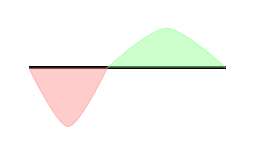
\begin{tikzpicture}[scale=0.5]
     \draw[thick] (0,0) -- (5,0);
     \filldraw[red!40, semitransparent] plot [smooth] coordinates {(0,0) (1,-1.5) (2,0)};
     \filldraw[green!40, semitransparent] plot [smooth] coordinates{(2,0) (3.5,1) (5,0)};
 \end{tikzpicture}
 \end{center}


\begin{align}
    \pdv{p(T,V)}{V} = 0 \quad &, \quad \pdv[2]{p(T,V)}{V}=0\\
    &\Longrightarrow p_k, \ T_k, \ V_k
\end{align}

\begin{center}
    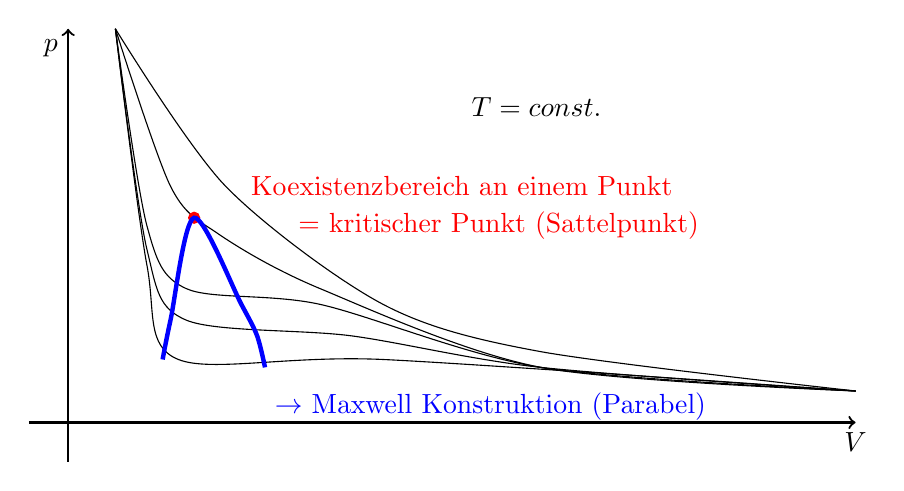
\begin{tikzpicture}
        \draw[->,thick] (-0.5,0) -- (10,0) node[anchor=north]{$V$};
        \draw[->,thick] (0,-0.5) -- (0,5) node[anchor=north east]{$p$};
        \coordinate (a) at (0.6,5);
        \coordinate (b) at (10,0.4);
        \draw plot [smooth] coordinates {(a) (2,3)  (4,1.5) (6,0.9) (b)};
        \draw plot [smooth] coordinates{(a) (1,2) (1.4,0.8) (4,0.8) (b)};
        \draw plot [smooth] coordinates{(a) (1,2.2) (1.5,1.3)(3.6,1.1) (6,0.7) (b)};
        \draw plot [smooth] coordinates{(a) (1,2.5) (1.5,1.7)(3.2,1.5) (6,0.7) (b)};
        \draw plot [smooth] coordinates{(a) (1.3,3) (1.9,2.4)(3.2,1.7) (6,0.7) (b)};
        \draw (5,4) node[anchor=west]{$T=const.$};
        \filldraw[red] (1.6,2.6) circle (2pt);
        \draw[red] (2.2,3) node[anchor=west]{Koexistenzbereich an einem Punkt};
        \draw[ultra thick,blue] plot [smooth] coordinates{(1.2,0.8) (1.3,1.3) (1.6,2.6) (2.2,1.5) (2.4,1.1) (2.5,0.7)};
        \draw[red] (2.8,2.5) node[anchor=west]{= kritischer Punkt (Sattelpunkt)};
        \draw[blue](2.5,0.2) node[anchor=west]{$\rightarrow$ Maxwell Konstruktion (Parabel)};
    \end{tikzpicture}
    \begin{tikzpicture}[scale=0.9]
        \begin{axis}[
        axis lines = left,
        axis line style={my axis},
        xmin=0, xmax = 6,
        ymin=0, ymax = 3.5,
        xtick=\empty, ytick=\empty,]
        \addplot[domain=1:5, samples=100, color=blue,]{exp(x/4)-0.5};
    \end{axis}
    \draw (7,0) node[anchor=west]{$T$};
    \draw (0,5.5) node[anchor=east]{$p$};
    \filldraw[red] (5.7,4.8) circle (3pt)  node[anchor=west]{kritischer Punkt};
    \draw (6,4) node[anchor=west]{$\rightarrow$ darüber kein Phasenübergang mehr};
    \draw[black!40] (3.5,2.5) node[anchor=west]{gasförmig};
    \draw[black!40] (2,3) node[anchor=west]{flüssig};
    \draw (6,2) node[anchor=west]{$\rightarrow$ Stehenbleiben an Dampfdruckkurve};
    \draw (6.5,1.2) node[anchor=west]{$\widehat{=}$ Koexistenzgerade};
    \end{tikzpicture}
\end{center}

\paragraph{Bemerkungen:}
\begin{itemize}
    \item Für $T>T_k$ sind Flüssigkeit und Gas nicht unterscheidbar
    \item Phasenübergang 1.Ordnung: Durchgang durch Dampfdruckkurve (z.B. $T=const$, und $p$ varriert)
    \begin{itemize}
        \item z.B. $T=const.$ und $p$ variiert
        \item $V_{fl} \neq V_{gas}$ ; $V(p)=\left(\pdv{G}{p}\right)_{T,N}$
        \item 1.Ordnung, da $V(p)$ unstetig
        \item Umwandlungswärme
    \end{itemize}
    \item Phasenübergang 2.Ordnung: kritischer Punkt (z.B. $\Delta V = V_{gas}-V_{fl}$ als Funktion von $T$)
    \begin{itemize}
        \item bei $T>T_k: \ \Delta V = 0$\\
        bei $T<T_k: \ \Delta V > 0$ mit $\lim_{T\rightarrow T_k} \Delta V = 0$
        \item 2. Ordnung, da $\Delta V(T)$ stetig, kontinuierlicher Phasenübergang
        \item keine Umwandlungswärme
    \end{itemize}
\end{itemize}


\subsubsection{Osmotischer Druck}
\begin{definition}{Halbdurchlässige Membran}
    Lösungsmittel geht durch, gelöster Stoff nicht\\
    Beispiel: Zellwand
\end{definition}
\begin{center}
\begin{tikzpicture}[scale=0.5]
    \draw[ultra thick] (0,5) -- (0,0) -- (10,0) -- (10,5);
    \fill[semitransparent, blue!20] (0,0) rectangle (10,4);
    \fill[semitransparent, blue!20] (4.5,4) rectangle (5.5,5);
    \draw (8,1) node{A};
    \draw[thick] (4.5,6) -- (4.5,3) -- (3,3) -- (3,2) -- (7,2) -- (7,3) -- (5.5,3) -- (5.5,6);
    \fill[pattern=dots] (4.5,5) -- (4.5,3) -- (3,3) -- (3,2) -- (7,2) -- (7,3) -- (5.5,3) -- (5.5,5) -- cycle;
    \draw (5,2.5) node{B};
    \draw[blue!40] (0.5,0.5) node[anchor=west]{\footnotesize Lösungsmittel};
\end{tikzpicture}
\end{center}


Theorie verdünnter Lösungen
\begin{align}
    P^B(T,\mu , n_s)=P_{Lös}(T,\mu)+\underbrace{n_skT}_{\text{gelöster Stoff verhält sich wie ideales Gas}}+O(n^2_s)\\
    n_s=\frac{N_s}{V_B}=\frac{\text{Zahl der gelösten Teilchen}}{\text{Volumen B}}
\end{align}
\begin{definition}{Osmotischer Druck (van´t Hoffsches Gesetz)}
\begin{align}
    p_{Osm}=p^B-p^A=n_skT
\end{align}
\end{definition}
(GG: $p_L$ muss in A und B gleich sein)
\subsubsection{Siedepunkterhöhung, Gefrierpunkterniedrigung}
2 Phasen:
\begin{enumerate}
    \item Phase A, flüssig, Lösungsmittel und gelöster Stoff mit $n_s=\frac{N_s}{V_A}$
    \item Phase B, gasförmig oder fest (nur Lösungsmittel)
\end{enumerate}
$n_s=0$: Koexistenz $p=p^A_{Lös}(T,\mu)\overset{!}{=} p^B_{Lös}(T,\mu)$\\
$n_s > 0$: verschobene Koex.-Kurve $p'=p^A_{Lös}(T',\mu ')+n_skT'\overset{!}{=} p^B_{Lös}(T',\mu')$\\
Gibbs-Duhen
\begin{align}
    SdT-Vdp+Nd\mu=0 \Rightarrow dp=\frac{S}{V}dT +\frac{N}{V}d\mu 
\end{align}
Für Phase A:
\begin{align}
    \Delta p = p'-p=\frac{S^A}{V^A}\Delta T+ \frac{N^A}{V^A}\Delta\mu + \frac{N_s}{V^A}k(T+\Delta T)
    \label{Phase_A}
\end{align}
Für Phase B:
\begin{align}
     \Delta p = p'-p=\frac{S^B}{V^B}\Delta T+ \frac{N^B}{V^B}\Delta\mu
     \label{Phase_B}
\end{align}
$\frac{V^A}{N^A}\cdot$Glg \ref{Phase_A} $-\frac{V^B}{N^B}\cdot$Glg \ref{Phase_B}:
\begin{align}
    \left(\frac{V^A}{N^A}-\frac{V^B}{N^B}\right)\Delta p = \underbrace{\left(\frac{S^A}{N^A}-\frac{S^B}{N^B}\right)}_{-\frac{1}{T}q_{A\rightarrow B}}\Delta T + \underbrace{\frac{N_s}{N_A}}_{c_s}kT
\end{align}
\begin{multicols}{2}
    $p_{A\rightarrow B}$: Umwandlungswärme pro Teilchen $A\rightarrow B$\\
    $c_s$: Konzentration

\begin{center}
    \begin{tikzpicture}[scale=0.3]
        \begin{axis}[
        axis lines = left,
        axis line style={my axis},
        xmin=-1, xmax = 6,
        ymin=0, ymax = 3.5,
        xtick=\empty, ytick=\empty,]
        \addplot[domain=1:4.5, samples=100,]{exp(x/4)-0.24};
        \addplot[domain=0:1, samples=100,]{1/x};
        \addplot[domain=1:4.5, samples=100, color=black!40,]{exp((x+0.2)/4)-1};
        \addplot[domain=0:1, samples=100, color=black!40,]{1/(x+0.2) -0.45};
    \end{axis}
    \draw (7,0) node[anchor=west]{$T$};
    \draw (0,5.5) node[anchor=east]{$p$};
    \filldraw (1.95,1.7) circle (3pt);
    \filldraw[black!40] (1.95,0.65) circle (3pt);
    \draw[blue,->] (1.35,4) -- (1.15,4);
    \draw[blue,->] (3.2,2.5) -- (4.3,2.5);
    \draw[blue,->] (3.2,2.5) -- (3.2,1.5);
    \end{tikzpicture}
\end{center}
\end{multicols}

Sei $\Delta p = 0$:
\begin{align}
    \frac{\Delta T}{T}=c_s\frac{kT}{q_{A\rightarrow B}}
\end{align}
Fallunterscheidung:
\begin{enumerate}
    \item $q_{fl\rightarrow g}>0$ Siedepunkterhöhung
    \item $q_{fl\rightarrow fest} <0$ Gefrierpunkterhöhung (Deswegen wird im Winter Salz gestreut)
\end{enumerate}
sei $\Delta T = 0$:\\
B sei ideales Gas mit $\frac{V_B}{N_B}>>\frac{V_A}{N_A}$ und $pV^B=N^BkT$ dann folgt
\begin{definition}{Dampfdruckerniedrigung}
    \begin{align}
        \frac{\Delta p}{p}= -c_s
    \end{align}
\end{definition}


\subsection{Wärmekraftmaschinen}
\begin{center}
    \begin{tikzpicture}[scale=0.6,
    sn/.style={rectangle, draw=black, fill=black!5, very thick, minimum size=1cm},
    ]
    \node[sn]   (WB1)                   {$T_1$};
    \node[sn]   (WB2) [below= of WB1]   {$T_2$};
    \node[sn]   (WKM) [right= 5cm of {$(WB1)!0.5!(WB2)$}]   {WKM};
    \node       (System) [right= 3cm of WKM] {};
    \draw[->] (WB1.east) -- (WKM.west) node[above= 0.1 of {$(WB1.east)!0.5!(WKM.west)$}]{$Q_1$};
    \draw[<-] (WB2.east) -- (WKM.west) node[below= 0.1 of {$(WB2.east)!0.5!(WKM.west)$}]{$Q_2$};
    \draw[->] (WKM.east) -- (System.west) node[above= 0.1 of {$(WKM.east)!0.5!(System.west)$}]{$W$};
    \end{tikzpicture}
\end{center}

\textbf{Wärme von 1 $\rightarrow$ Arbeit $(T_1>T_2)$}\\
Bilanzgleichung für eine Periode des
Kreisprozesses:
\begin{enumerate}
    \item Wärmeentzug von Bad 1 : $Q_1 = -T_1\Delta S_1>0 \Rightarrow \Delta S_1<0$
    \item Wärmeabgabe an Bad 2 : $Q_2 = T_2 \Delta S_2 > 0 \Rightarrow \Delta S_2 > 0$
\end{enumerate}
Anwendung der Hauptsätze:
\begin{enumerate}
    \item HS: $\Delta U_{WKM}=Q_1-Q_2-W=0$
    \item HS: $\Delta S_{Gesamt}= \Delta S_1 + \Delta S_2 + \underbrace{\Delta S_{WKM}}_{=0} + \underbrace{\Delta S_{\text{Speicher Arbeit}}}_{\approx 0}\geq 0$
\end{enumerate}
\begin{align}
    \Delta S_2 \geq -\Delta S_1 \enspace (\text{reversibel }\Delta S_2 = -\Delta S_1)
\end{align}
Wirkungsgrad:
\begin{align}
    \eta = \frac{\text{abgegebene Arbeit}}{\text{benutzte Wärme}}=\frac{W}{Q_1}=\frac{Q_1-Q_2}{Q_1}=1-\frac{T_2\Delta S_2}{T_1(-\Delta S_1)}\leq 1-\frac{T_2}{T_1}
\end{align}
Carnot: Für alle reversiblen WKM gilt
\begin{align}
    \eta_{rev}= 1-\frac{T_2}{T_1}
\end{align}
\begin{beispiel}{Wärmekraftmaschinen}
\begin{itemize}
    \item Praxis:\\
            Reversibilität $\Rightarrow$ quasistatisch $\Rightarrow$ beliebig langsam $\Rightarrow$ geringe Leistung (meist 30\%-40\% von $\eta_{rev}$)
    \item Perpetuum Mobile 2.Art:
    \begin{enumerate}
        \item HS erfüllt, $W=0_1$, $Q_2=0$
        \item HS : $\Delta S_{Gesamt} = \underbrace{\Delta S_1}_{<0} \geq 0$ !!!
    \end{enumerate}
    \item Kühlschrank:\\
        Arbeit $\rightarrow$ Abkühlung von 1: $T_1<T_2$
        \begin{align}
            W=Q_1-Q_2&=-T_1\Delta S_1-T_2\Delta S_2\\
            &= -T_1(\Delta S_1 + \Delta S_2)-(T_2-T_1)\Delta S_2 < 0
        \end{align}
        $\Rightarrow$ es muss Arbeit zugeführt werden.\\
        Effizenz:
        \begin{align}
            \epsilon = \frac{\text{extrahierte Wärme}}{\text{zugeführte Arbeit}}=\frac{Q_1}{-W}=\frac{Q_1}{Q_2-Q_1}\leq \frac{T_1}{T_2-T_1}
        \end{align}
        Bem.:
        \begin{align}
            T_1 \rightarrow 0 \Rightarrow \epsilon \rightarrow 0 \quad\widehat{=} \quad\text{3.HS}
        \end{align}
    \item Wärmepumpe:\\
        Arbeit $\rightarrow$ Erwärmung von 2 $T_1<T_2$, gleicher Prozess wie beim Kühlschrank aber anderes Ziel\\
        Effizienz:
        \begin{align}
            \Tilde{\epsilon}=\frac{\text{zugeführte Wärme}}{\text{zugeführte Arbeit}}=\frac{Q_2}{-W}=...\leq \frac{T_2}{T_2-T_1}
        \end{align}
\end{itemize}
\end{beispiel}
